\documentclass[a4paper,11pt]{article}
\usepackage{graphicx}
\usepackage{csquotes}
\usepackage{hyperref}
\usepackage[a4paper,left=1.5cm,right=1.5cm,top=2cm,bottom=2cm]{geometry}
\graphicspath{ {figures/} }
\begin{document}

\begin{titlepage}
    \centering
    {\scshape\LARGE CMPT 732 Project\par}
    \vspace{1cm}
    {\Large Kyle Demeule \\ 301083503\par}
\end{titlepage}

\section*{Introduction}
Amazon is the largest online-retailer in the United States, and recently surpassed Walmart as the most valuable retailer in the U.S. by market capitalization. One of the pioneers of online-retail, Amazon had to develop techniques that would make shoppers comfortable in abandoning physical retail locations to purchase their goods online. One of these techniques was to allow anyone to review any item. Since it's inception, Amazon.com has become the largest source of internet consumer reviews. But how do customers utilize Amazon reviews? Allow me to provide a use case:

You know you want a particular type of product (e.g. coffee grinder), but you don't know anything about the best brands or models for this type of product. So you go to Amazon.com, and search for \enquote{coffe grinder}. You sort the results by either \enquote{relevance} or \enquote{average customer review}. You pick and item within your price range that has a 4+ average review score with ~20+ reviews. You click that item, look at a few pictures, and then scroll down to the \enquote{Most Helpful Reviews} section. You read 1-2 of them, they're well written and positive, so you purchase the product.

This type of approach is common among Amazon customers I've talked to. It also relies heavily on the user submitted reviews, specifically their aggregate and helpfulness scores. But is it a good idea? I'll evaluate each portion 

\section*{Data Set}
For this report I will be analyzing approximately 83 million amazon reviews from May 1996 to July 2014, and metadata on approximately 9 million products. The dataset was collected by Julian McAuley, and information is available \href{http://jmcauley.ucsd.edu/data/amazon/}{here}. The reviews are in json form and compressed are about 18GB. The metadata compressed is about 3GB.

\section*{Amazon Review}
A user submitted review on Amazon has several components. The first is a star rating from 1 to 5. Next is a summary of the review, the main review text, and then a helpfulness score. User's can vote on a review in a yes/no fashion, stating whether they found the review helpful.

\section*{Review Scores}
When examine user reviews it's useful to know how they are distributed. Before starting this project my expectation was something like a smile, peaks at 1 and 5, valley at 3. The actualy distribution is a little surprising:

\begin{center}
    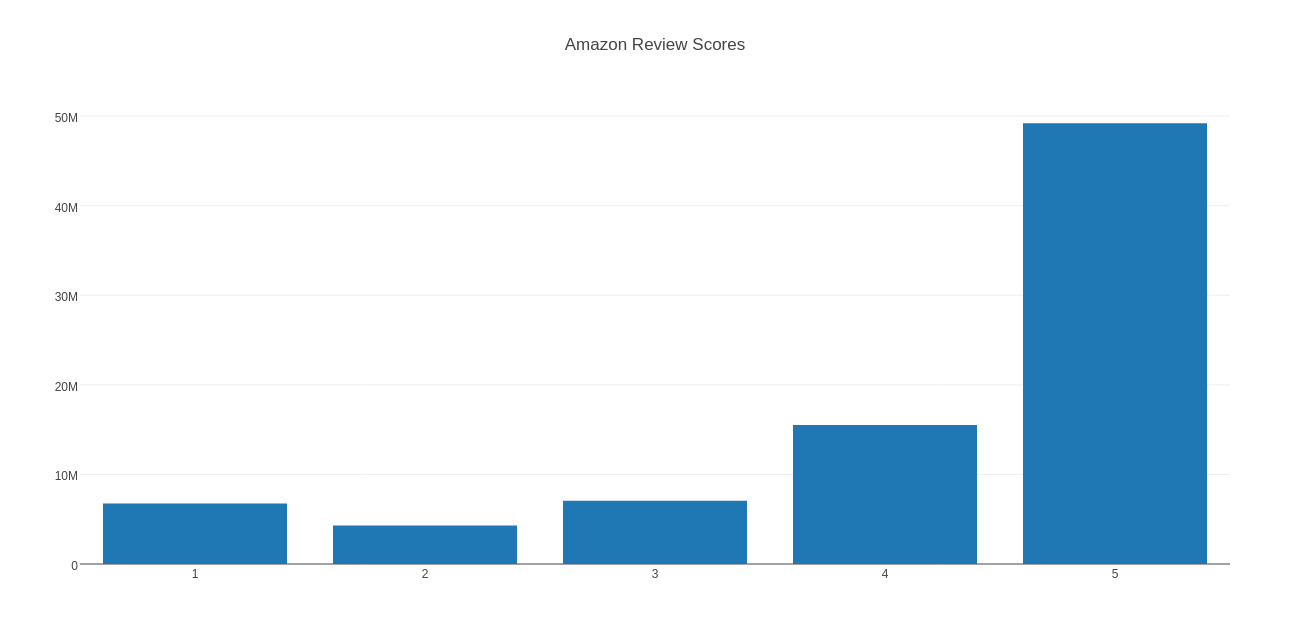
\includegraphics[scale=0.25]{score_histogram.png}
\end{center}

As we can see the reviews are intensily skewed towards 5 star reviews. In fact they make up around \textbf{42\%} of all reviews on Amazon. This distribution gives the average score of an amazon review as \textbf{4.16}, much higher than I had anticipated. However this does not mean that the average product score is 4.16, it's possible than a large number of the 5-star reviews go to the same sub-group of products, so it's worthwhile to investigate the distribution of average product review scores:

\begin{center}
    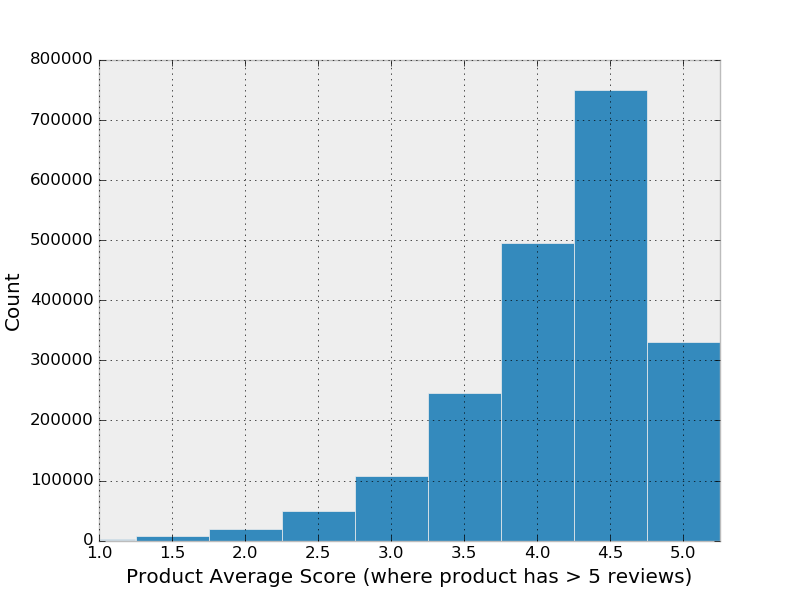
\includegraphics[scale=0.65]{starbins_gt_5.png}
\end{center}

It's worth noting that this chart only includes products with at least 5 reviews. When you include products with less you see large spikes around the X.0 and X.5 bins, which are not interesting (this is because if a product only has 1-2 reviews, it's average review score must end in X.0 or X.5, and there are a lot of products with < 3 review scores). In the interest of finding interesing trends, and since most consumers would ignore products with little or no reviews, I will use a minimum product review condition.

Again we see a significant right skew to the distribution, with a peak at around the 4.5 mark. These bin sizes were picked for a very important reason. The Amazon UI will never actually tell you the true average score of a product, it only shows it in stars. The lowest level of granularity that the Amazon UI provides is a half star, so each of these bins corresponds to what the product would get rounded to at the center of the bin. A breakdown of the ranges:

\begin{center}
    \begin{tabular}{l l l l}
    \textbf{Range} & \textbf{Stars} & \textbf{Count} & \textbf{Percent} \\
    \hline
    1.00-1.24 & 1.0 & 1831      & 0.09\% \\
    1.25-1.74 & 1.5 & 7702      & 0.38\% \\
    1.75-2.24 & 2.0 & 19894     & 0.99\% \\
    2.25-2.74 & 2.5 & 48707     & 2.43\% \\
    2.75-3.24 & 3.0 & 107941    & 5.37\% \\
    3.25-3.74 & 3.5 & 245643    & 12.23\% \\
    3.75-4.24 & 4.0 & 495257    & 24.65\% \\
    4.25-4.74 & 4.5 & 750529    & 37.36\% \\
    4.75-5.00 & 5.0 & 331302    & 16.49\% \\
    \end{tabular}
\end{center}
What we see here is around \textbf{53\%} of products with over five reviews will show as either 4.5 or 5 stars. At least \textbf{78\%} of products with over five reviews will show as 4, 4.5, or 5 stars. This was quite shocking to me, as I used to have the impression the a product with 4.5 or 5 stars was essentially perfect, and anything with 4 or over was amazing. There are certain types of stores that only sell products that meet a certain quality threshold, and don't carry cheaper goods (e.g. MEC). Amazon is not one of these. Their logo literally implies they carry everything from A to Z, and except in terms of legality they will sell any product. The notion that nearly 4 out of 5 products on Amazon are \enquote{amazing} is ridiculous and should be abandoned. Unless you believe that 78\% of products on amazon would meet your buying standard the star rating of a product on Amazon gives a false sense of security and should not be relied upon.


\section*{Helpfulness}
Amazon allows users to mark whether they found a review helpful or not, giving each review a helpfulness score. This score is used to pick between 1 and 8 reviews to highlight and be shown on a products page. I wondered how the distribution of reviews Amazon chose to show on a products main page compared to the total reviews for the product. Unfortunately this data was not in my origin dataset, so I had to do some additional processing. I picked 2000 items at random, and retrieved the reviews Amazon displayed for them. I also retrieved each products overall count of reviews for each star rating. I compare the distribution of shown helpful reviews and total reviews here:
\begin{center}
    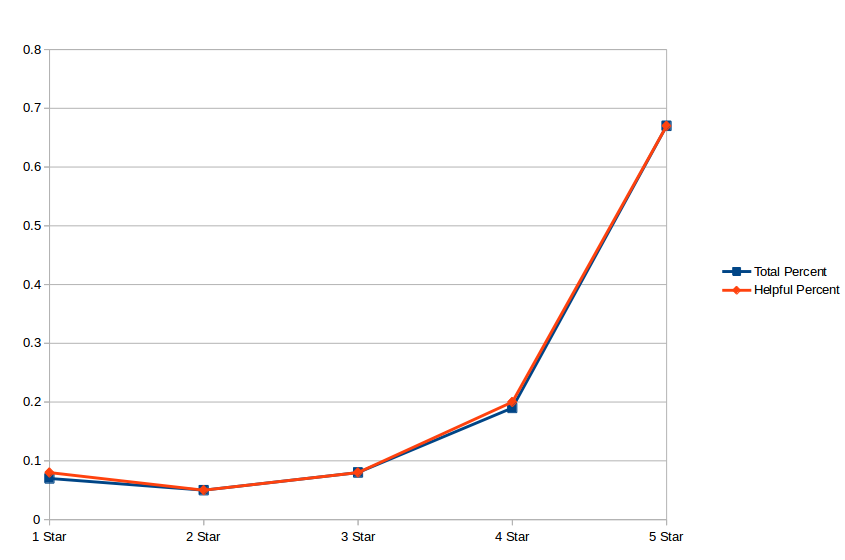
\includegraphics[scale=0.5]{helpfulness.png}
\end{center}
As we can see, they are essentially the same. This can be taken as a good thing or a bad thing. The good aspect is that the \enquote{helpful} reviews don't inflate the perception of all the reviews for the product, they are fair representation of the rest of the reviews. The bad part is they dont inflate the reviews because the reviews were already inflated. If you randomly sampled reviews you'd see the same thing. And according to previous research, that's essentially what you're doing. In 2009, Bing Liu from the University of Illinois did a study on spam in Amazon reviews. He developed a model that could predict spam to an 80\% accuracy. He analyzed the spammy-ness of reviews with high helpfulness scores to reviews with low helpfulness scores and found \textbf{no difference}. And this makes sense, how easy is it to mark a review as heplful? How easy would it be to game that system? (not to mention how reviews with a high number of helpful points are more visible and thus more likely to get more helpful votes)

In effect, highlighting helpful reviews is almost equivalent to highlighting random reviews, and how helpful is that?

\section*{Alternate Solution}
My original instinct was that this must be caused by spam. Fraudulent reviews to inflate the scores of products. But if we analyze studies done on fraudulent reviews on Amazon, this might not be the case. Recall Bing Liu's model from earlier? ~80\% accuracy at identifying spam reviews, but when they applied that to their entire data set they only found ~1\% of reviews could be considered spam. Going back to our original distribution diagram, nearly 50 million reviews are 5-stars. If 1\% of reviews are spam, then in the best case scenario we could remove ~800,000 reviews from the 5-star group. In the immortal words of the NASA guy from Armaggedon, that's like firing a BB gun at a freight train. We need a different approach.

\section*{Results}
If you have a cluster that is in a circulare shape, and have an outlier that is right in the middle:
\begin{center}
    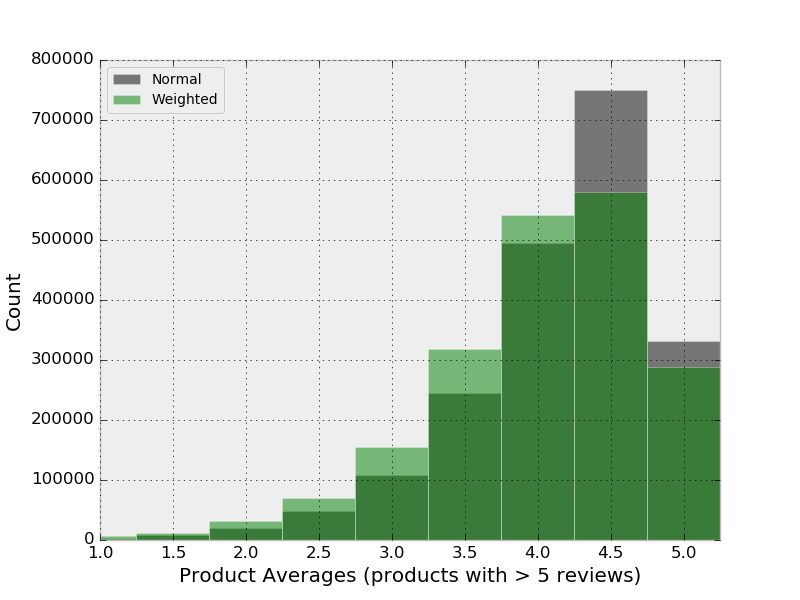
\includegraphics[scale=0.65]{normascore_vs_regular.png}
\end{center}
The angle for the outlier could be anything, and could be very large, even larger than some of the points in the clusters.
\begin{center}
    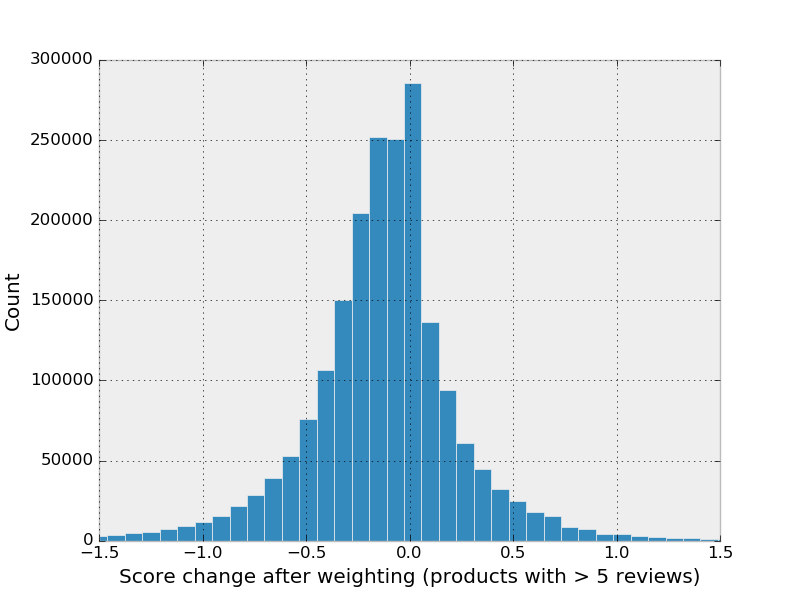
\includegraphics[scale=0.65]{normascore_changes.png}
\end{center}
The angle for the outlier could be anything, and could be very large, even larger than some of the points in the clusters.

\section*{Usage}
If you have a cluster that is in a circulare shape, and have an outlier that is right in the middle:

\section*{Dataset}
If you have a cluster that is in a circulare shape, and have an outlier that is right in the middle:

\section*{Technology}
If you have a cluster that is in a circulare shape, and have an outlier that is right in the middle:

\end{document}